\documentclass[linenumbers]{aastex631}
\usepackage{graphicx}
\newcommand{\vdag}{(v)^\dagger}
\newcommand\aastex{AAS\TeX}
\newcommand\latex{La\TeX}

\begin{document}

\title{ASTR400B Research Proposal}

\author{Peter Hartman}
\affiliation{University of Arizona}

\section{Introduction} \label{sec:intro}
I propose to study the topic of the dark matter halo evolution of the M31/Milky Way Merger remnant, and particularly the density profile of the dark matter halo.

Due to dark matter's purely gravitational interaction with baryons, its density profile is the most important component of dark matter's effect on galaxy evolution. The density profile of the halo is critical for the baryonic matter within the halo, as it determines the rotation rate of the galaxy and provides much of the mass to bind it. As such, the galactic structures we see heavily depend on the dark matter halo that they are embedded in.

While dark matter halos have a surprisingly universal spherically-averaged density profile, the triaxial nature of dark matter halos are important to consider. \cite{Meneghetti} determined that triaxial halos are necessary to match with CDM modeling, and the halo shape has an effect on stellar streams and nearby satellites due to the alteration of the potential.

There remains an open question regarding the effect produced by mergers on dark matter halos and how the density profile and shape changes with mergers.

\cite{Abadi} showed that the dark matter halo reacts and changes shape due to the baryonic matter it influences. Inside of stellar mergers, these effects become very important, as a large amount of baryonic matter is interacting with both halos, affecting their density profiles. \cite{Despali} determined that halos will become elongated along the merger axis, and then smooth out to a spherical shape over time. I hope to determine the effect induced by a merger on halo shape and distribution by building figures similar to those of Figure \ref{fig:1}.


\begin{figure}[h!]
    \centering
    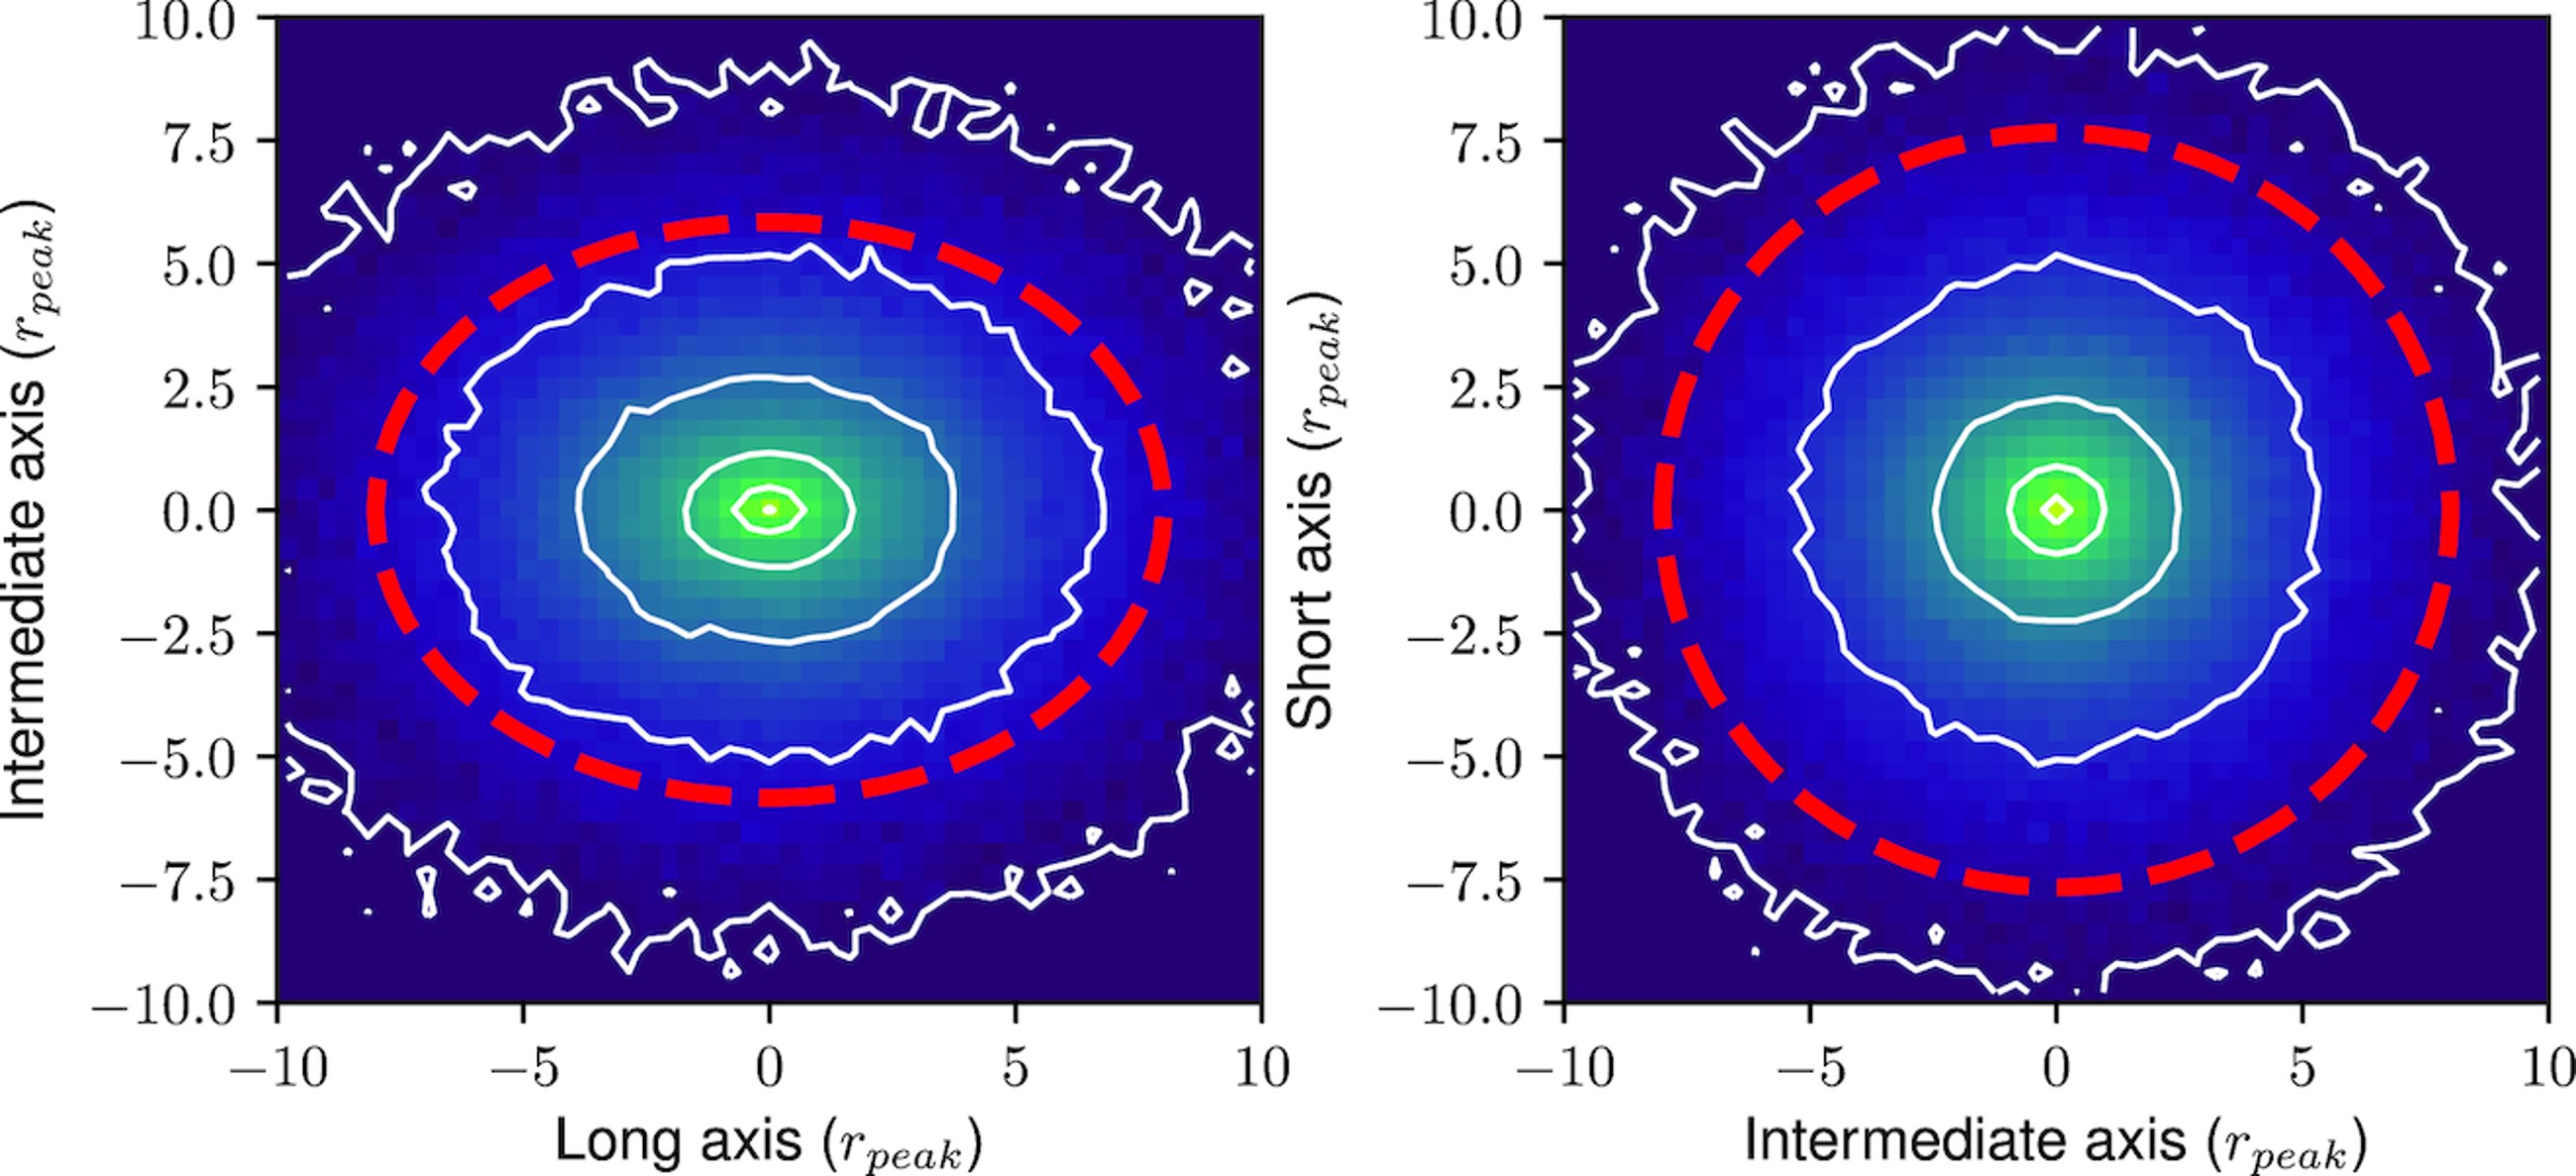
\includegraphics[width=\textwidth]{DrakosFig.jpg}
    \caption{A plot of isodensity contours on a dark matter halo after a merger. I hope to reproduce this type of figure to test changes in the dark matter halo profile and shape. The red dashed lines indicate the measured shape ratio, while the white contours show the expected shape. Figure from \cite{DrakosA}}
    \label{fig:1}
\end{figure}
\section{Proposal}

I will be addressing the question of how the density distribution changes after the merger. 

This will be done with a combination of old and new codes. The initial conditions are given in the simulation data, following a Hernquist profile. I will use the final timestep in simulation at SnapNumber 800 to determine the final state after the merger remnant has relaxed. The new code will be written to determine the shape of the halo, by creating isodensity contours for the halo in the xy, yz, and xz planes. I will then fit those contours with ellipses and determine the a, b, and c axes in both the initial and final states. A triaxial halo will have different values of a, b, and c, and the spherical profiles will have equal a, b, and c.

I expect the initial halos to be a spherical shape, as they are set up in simulation based on a Hernquist profile. I expect the final halo to still follow a Hernquist profile when spherically averaged, but to be elongated along the merger axis, as the interaction between M31's halo and the Milky Way's halo stretches the combined distribution.

\begin{figure}[h]
    \centering
    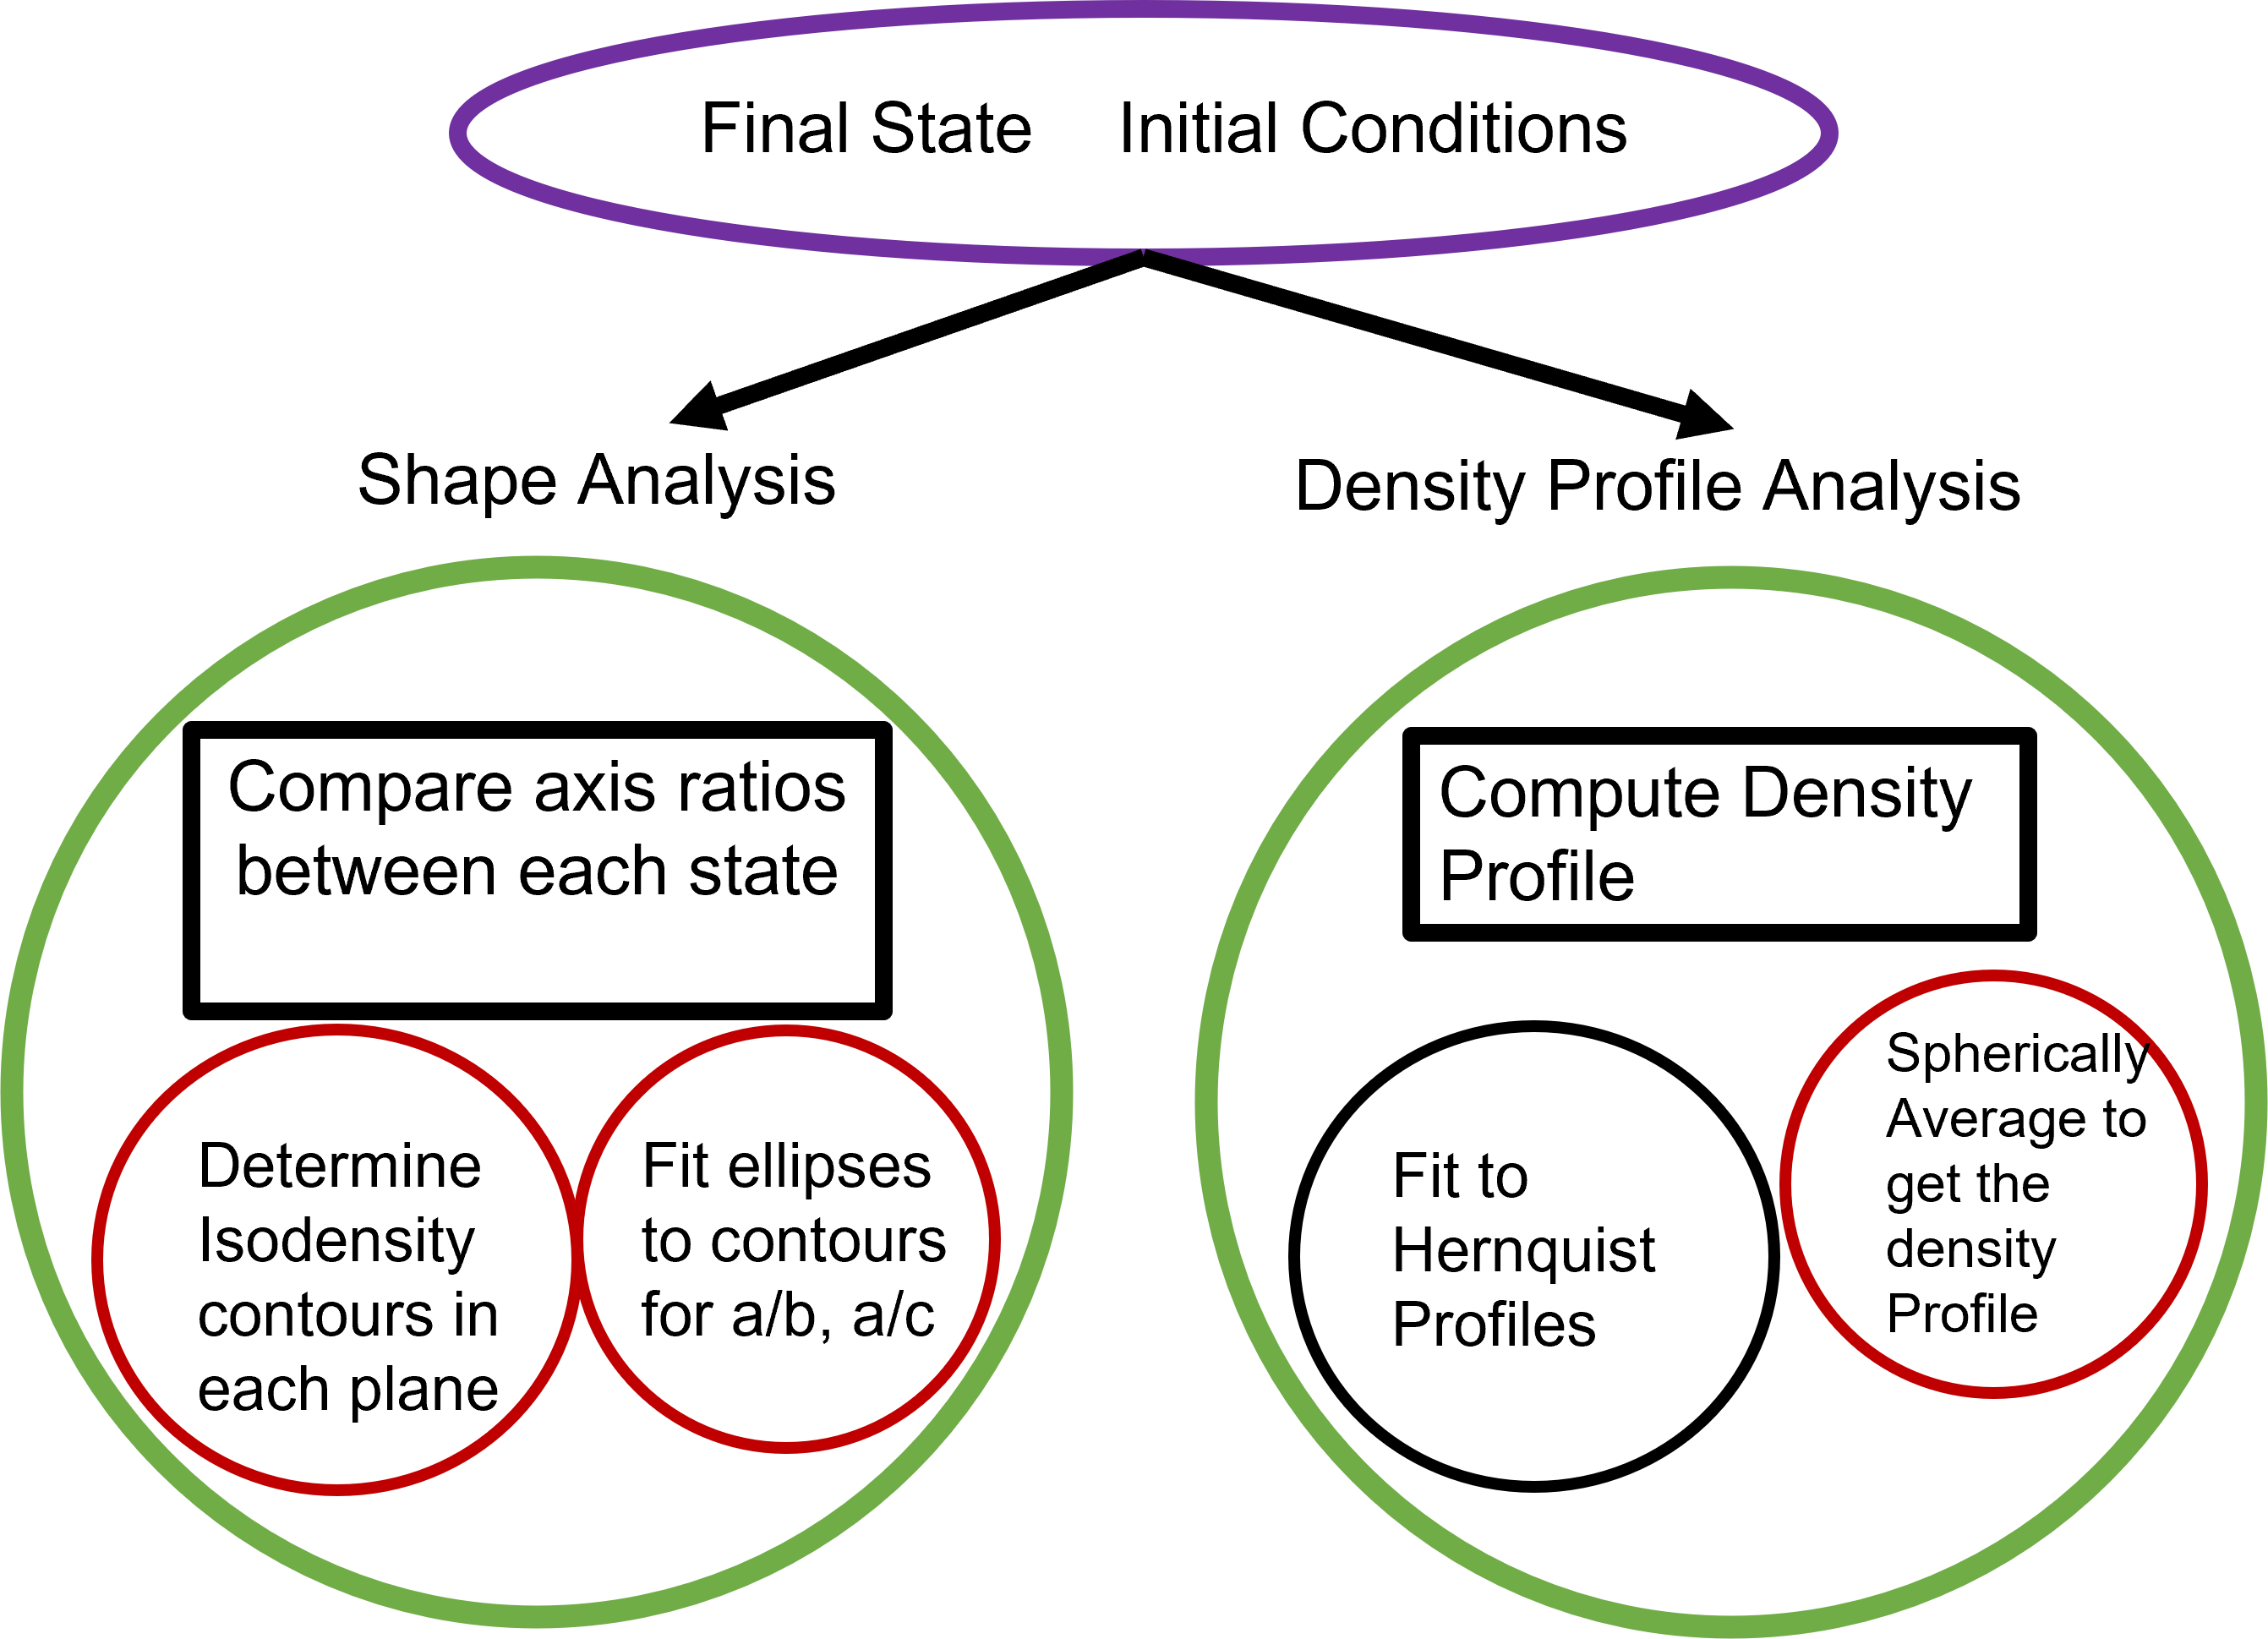
\includegraphics[width=\textwidth]{MethodsFlowchart400B.png}
    \caption{A general overview of my process for analysis. The purple borders indicate inputs, the green borders indicate broad analysis, and each bubble shows the goal in a black square and the necessary steps to follow in circles. New codes will be needed for the red circles and black circles indicate steps that can be done with existing codes.}
    \label{fig:2}
\end{figure}

\bibliography{sample631}

\end{document}